\documentclass[11pt]{article}

\usepackage[margin=1in]{geometry}
\usepackage{iftex}
\ifXeTeX
  \usepackage{fontspec}
  \setmainfont{Latin Modern Roman}
  \usepackage{xeCJK}
  \setCJKmainfont{Noto Serif CJK SC}
  \setCJKsansfont{Noto Sans CJK SC}
  \setCJKmonofont{Noto Sans Mono CJK SC}
  \newCJKfontfamily\zhfont{Noto Serif CJK SC}
\else\ifLuaTeX
  \usepackage{fontspec}
  \setmainfont{Latin Modern Roman}
  \usepackage{luatexja-fontspec}
  \setmainjfont{Noto Serif CJK SC}
  \newjfontfamily\zhfont{Noto Serif CJK SC}
\else
  \usepackage[T1]{fontenc}
  \usepackage{lmodern}
\fi\fi
\usepackage{microtype}
\usepackage{amsmath,amssymb,amsthm,mathtools}
\usepackage{booktabs,array,longtable,tabularx}
\usepackage[dvipsnames]{xcolor}
\usepackage{graphicx}
\usepackage{tikz}
\usetikzlibrary{arrows.meta,positioning,decorations.pathreplacing}
\usepackage[numbers,sort&compress]{natbib}
\usepackage{hyperref}
\usepackage{xurl}
\usepackage{enumitem}
\usepackage{caption}

\definecolor{FlowBlue}{HTML}{0072B2}
\definecolor{FlowTeal}{HTML}{009E73}
\definecolor{FlowOrange}{HTML}{E69F00}
\definecolor{FlowRed}{HTML}{D55E00}

\hypersetup{
  colorlinks=true,
  linkcolor=MidnightBlue,
  citecolor=ForestGreen,
  urlcolor=BrickRed,
  pdftitle={One Clock, One Characteristic},
  pdfauthor={Liang Wang}
}

\newtheorem{theorem}{Theorem}
\newtheorem{proposition}[theorem]{Proposition}
\newtheorem{corollary}[theorem]{Corollary}
\newtheorem{lemma}[theorem]{Lemma}
\theoremstyle{definition}
\newtheorem{definition}[theorem]{Definition}
\theoremstyle{remark}
\newtheorem{remark}[theorem]{Remark}

\newcommand{\R}{\mathbb{R}}
\newcommand{\Z}{\mathbb{Z}}
\newcommand{\N}{\mathbb{N}}
\newcommand{\F}{\mathbb{F}}
\newcommand{\C}{\mathbb{C}}
\newcommand{\Spec}{\operatorname{Spec}}
\newcommand{\Fix}{\operatorname{Fix}}
\newcommand{\Tr}{\operatorname{Tr}}
\newcommand{\cP}{\mathcal{P}}
\newcommand{\e}{\mathrm{e}}
\newcommand{\proved}{\textsf{PROVED}}
\newcommand{\modelchoice}{\textsf{MODELING CHOICE}}
\newcommand{\nottest}{\textsf{NOT TESTABLE}}
\newcommand{\refuted}{\textsf{REFUTED}}
\newcolumntype{Y}{>{\raggedright\arraybackslash}X}
\newcolumntype{L}[1]{>{\raggedright\arraybackslash}p{#1}}

\title{\textbf{One Clock, One Characteristic:}\\
A Frobenius-Suspension Positive Control for Arithmetic Flow Zeta Functions}
\author{Liang Wang\\
\small School of Artificial Intelligence and Automation,\\[-2pt]
\small Huazhong University of Science and Technology, Wuhan 430074, P.R. China\\
\small \texttt{wangliang.f@gmail.com}}
\date{13 August 2026}

\begin{document}
\maketitle

\begin{abstract}
An exact match between an orbit product and an Euler product is informative
only when the primitive objects and their clocks arise from a frozen
arithmetic dynamics.  We construct a positive control from arithmetic
Frobenius on the geometric points of
\(\mathbb P^1_{\F_2}\), equipped with the explicitly disclosed discrete
topology, and suspend it with constant roof \(\log 2\).  Closed points,
primitive Frobenius cycles, and primitive suspension orbits are then in
bijection, and the orbit attached to \(x\) has least period
\(\deg(x)\log 2=\log N(x)\).  We prove, first as a formal identity and then
analytically on \(\Re s>1\), that
\[
  \zeta_{\mathrm{orb}}(s)
  =Z(\mathbb P^1_{\F_2},2^{-s})
  =\frac{1}{(1-2^{-s})(1-2^{1-s})}.
\]
The repetition coefficient \(1/r\) and logarithmic weight \(\log N(x)\)
follow from the primitive factor and differentiation; neither is inserted as
a potential.  The same construction gives a sharp transfer boundary.  If
\(Q=\ell^f\) and \(n\log Q=r\log p\), unique factorization forces
\(p=\ell\), so one finite-field clock cannot produce rational-prime periods
across characteristics.  A disjoint union of circles of lengths \(\log p\)
does reproduce the Riemann Euler product, but the identical construction
compiles any prescribed locally finite length multiset and therefore fails
the arithmetic-origin gate.  Cohomological Frobenius determinants are kept
distinct from any transfer determinant of the neutral circle flow.  The
result is an exact native finite-field Route-A calibration, a proved rejection
for the Riemann target, and no Route-B or Hilbert--P\'olya claim.
\end{abstract}

\ifPDFTeX\else
\begin{center}
{\zhfont\bfseries 摘要}
\end{center}
{\zhfont
轨道乘积与 Euler 乘积的精确相等，只有在本原对象及其时钟由预先冻结的
算术动力系统产生时才具有判别力。本文取
\(\mathbb P^1_{\mathbb F_2}\) 几何点上的算术 Frobenius，明确赋予其离散
拓扑，并以 \(\log 2\) 为常值屋顶构造悬挂流。由此，闭点、本原
Frobenius 循环与本原流轨道一一对应；闭点 \(x\) 的最小周期为
\(\deg(x)\log2=\log N(x)\)。本文先在形式幂级数层面、再在
\(\Re s>1\) 的绝对收敛域内证明轨道 zeta 恰为
\(Z(\mathbb P^1_{\mathbb F_2},2^{-s})
=((1-2^{-s})(1-2^{1-s}))^{-1}\)。重复系数 \(1/r\) 来自本原因子的
对数展开，\(\log N(x)\) 则来自对悬挂时间参数求导，二者均非外加权重。
同一模型也给出严格的迁移边界：若 \(Q=\ell^f\) 且
\(n\log Q=r\log p\)，唯一分解迫使 \(p=\ell\)，故一个有限域时钟不能
跨特征生成全部有理素数周期。虽然逐个赋予长度 \(\log p\) 的互不相交
圆周能够精确写出 Riemann Euler 乘积，但该方法同样能够编译任意预设的
局部有限长度集合，因而在算术来源门槛处失败。本文严格区分上同调
Frobenius 行列式与中性圆周流可能具有的转移算子行列式。最终结论是：
该模型构成有限域原生目标的精确 Route-A 正控；对于 Riemann 目标则被
严格拒绝；本文不启动 Route B，也不提出 Hilbert--Pólya 声明。
}
\fi

\medskip
\noindent\textbf{Keywords:} arithmetic dynamics; Frobenius suspension;
Hasse--Weil zeta function; primitive orbit; constant roof; Euler-product
compiler; Route-A audit.

\section{Introduction}
\label{sec:intro}

Periodic-orbit formulas make arithmetic and dynamics look unusually close.
For a map with finitely many fixed points of each iterate, the Artin--Mazur
construction packages the fixed-point counts in an exponential generating
function \citep{ArtinMazur1965}.  In finite characteristic, the same fixed
points are rational points over extension fields, while closed points are
Frobenius orbits and the resulting product is the Hasse--Weil zeta function
\citep{Deligne1974,Milne2013}.  Suspending a return map turns discrete cycles
into closed flow orbits whose periods are roof sums, a standard bridge between
maps and flows \citep{ParryPollicott1990}.  These facts provide a rare setting
in which arithmetic source, primitive objects, clock, and zeta can all be
audited exactly.

Exact scalar agreement is nevertheless too weak to certify an arithmetic
flow.  Given a list of positive numbers \(L_j\), one may place a translation
flow on one circle of circumference \(L_j\) for each index \(j\).  Its
primitive-orbit product is automatically
\(\prod_j(1-\e^{-sL_j})^{-1}\).  Choosing \(L_p=\log p\) therefore writes the
Riemann Euler product into a phase space without discovering either primes or
their periods.  A useful positive control must succeed for a reason that this
universal compiler does not share.

This paper asks a deliberately narrow question.  For a fixed variety over a
finite field, does constant-roof Frobenius suspension give an exact,
locally compact continuous-time realization of its closed-point Euler
product, and what prevents the same one-clock construction from generating
the rational-prime divisor of \(\Spec\Z\)?  The concrete object is frozen
before analysis:
\[
  X=\mathbb P^1_{\F_2},\qquad
  S=X(\overline{\F}_2)_{\mathrm{disc}},\qquad
  F(a)=a^2,\qquad \tau=\log2.
\]
The subscript ``disc'' matters.  The arithmetic set and Frobenius action are
intrinsic, but the locally compact Hausdorff topology used for the suspension
is an imposed modeling choice.

Four theorem-level results follow.  First, closed points of \(X\), primitive
Frobenius cycles on \(S\), and primitive suspension orbits are in bijection;
the period is exactly \(\deg(x)\log2=\log N(x)\).  Second, the unweighted
orbit product equals the Artin--Mazur and Hasse--Weil zeta functions, and the
coefficients \(1/r\) and \(\log N(x)\) have explicit internal provenance.
Third, the Euler product converges absolutely exactly for \(\Re s>1\), while
the rational expression gives a separate meromorphic continuation with a
single-clock imaginary period.  Fourth, a fixed clock \(\log Q\), where
\(Q=\ell^f\), can meet a rational-prime-power clock only for \(p=\ell\).
The construction is consequently exact for its native finite-field target and
incompatible with the rational-prime target.

The contribution is a source-locked synthesis and falsification audit, not a
claim that the classical component identities are new.  It keeps three
determinant notions separate: the primitive-orbit Euler product, the
Artin--Mazur fixed-point zeta, and the \(\ell\)-adic cohomological Frobenius
determinant.  Their scalar values agree because they share an arithmetic
source.  No operator conjugacy or trace theorem identifies the last object
with a transfer operator of the neutral circle flow.

The Route-A consequence is correspondingly split.  Against the native
Hasse--Weil target, the object is an exact positive control through the
controlled-continuation layer.  Against Riemann \(\zeta/\xi\), it fails the
arithmetic support and determinant layers.  The disjoint-prime repair is
rejected even though its product is exact, because it reads the target divisor
and roof lengths into the phase space.  No Route-B layer is opened.

\section{Source lock, conventions, and research design}
\label{sec:lock}

\subsection{The frozen object}

Let \(F:S\to S\) be the permutation induced by the square map.  We use the
term \emph{arithmetic Frobenius} for the point action \(a\mapsto a^2\), in
the convention recorded by the Stacks Project \citep{Stacks03SL}.  Some
cohomological sources formulate trace identities using geometric Frobenius or
an inverse Galois convention.  We do not identify those actions by notation:
the return map in the flow is always the displayed square map.  Replacing it
by its inverse reverses each finite cycle but changes neither the cycle length
nor the unweighted orbit product.

Give \(S\) the discrete topology and let \(\Z\) act on \(S\times\R\) by
\begin{equation}
  n\cdot(a,u)=(F^n a,u-n\tau),\qquad \tau=\log2.
  \label{eq:action}
\end{equation}
The mapping torus and vertical flow are
\begin{equation}
  M_F=(S\times\R)/\Z,
  \qquad
  \phi^t[a,u]=[a,u+t].
  \label{eq:suspension}
\end{equation}
This is the constant-roof version of the standard suspension construction
\citep[Chap.~6]{ParryPollicott1990}.  The reference supplies the convention;
the topology of this noncompact countable-discrete base is proved directly in
Section~\ref{sec:orbits}.

The primitive-orbit zeta is frozen as
\begin{equation}
  \zeta_{\mathrm{orb}}(s)
    :=\prod_{\gamma\in\cP(M_F)}
      \left(1-\e^{-s\ell_\gamma}\right)^{-1}.
  \label{eq:orbit-zeta}
\end{equation}
Primitive multiplicity is one and orientation is positive vertical time.
There is no potential, phase, half-shift, stability denominator, fitted
prefactor, orbit cutoff, or numerical parameter.

\begin{table}[t]
\centering
\caption{Candidate lock and provenance.  The discrete topology is the main
additional modeling choice; the roof and orbit-zeta normalization are also
explicitly frozen.}
\label{tab:lock}
\small
\begin{tabularx}{\textwidth}{@{}p{0.23\textwidth}X p{0.20\textwidth}@{}}
\toprule
Field & Frozen value & Status\\
\midrule
Arithmetic scheme & \(\mathbb P^1_{\F_2}\) & intrinsic\\
Return map & \(F(a)=a^2\) & intrinsic\\
Base topology & discrete topology on \(X(\overline{\F}_2)\) & \modelchoice\\
Roof and clock & constant \(\tau=\log2\) & base-field norm\\
Orbit weight & one unweighted primitive factor & frozen convention\\
Target, native & \(Z(\mathbb P^1_{\F_2},2^{-s})\) & tested\\
Target, Riemann & \(\zeta(s)\) or \(\xi(s)\) & not assumed\\
Data use & exact algebra and deterministic controls & no zeros or fitting\\
\bottomrule
\end{tabularx}
\end{table}

\subsection{Evidence and falsification design}

The primary sources were checked through 13 August 2026.  Artin and Mazur
provide the fixed-point zeta definition and its finite-field power-map
example \citep{ArtinMazur1965}.  Deligne supplies the closed-point product,
Frobenius orbit dictionary, fixed-point counts, cohomological determinant,
and native functional-equation framework \citep{Deligne1974}.  Parry and
Pollicott supply standard suspension and orbit-zeta conventions
\citep{ParryPollicott1990}; the Stacks Project fixes Frobenius terminology and
finite residue-field facts \citep{Stacks01TF,Stacks03SL}; and Milne provides
an independent authoritative check of point-count and cohomological formulas
\citep{Milne2013}.

The source scope is deliberately asymmetric.  Hyperbolic suspension results
are not transferred to the present neutral, disconnected flow.  Conversely,
the cohomological rationality theorem is not called a transfer-operator
theorem for the circle suspension.  Statements about the topology, circle
decomposition, exact convergence boundary, clock obstruction, and universal
compiler are established below by direct proof.

Ten obligations were frozen before manuscript composition: completeness of
the closed-point dictionary; topological legitimacy; separation of primitive
and repeated orbits; agreement of the three native zeta conventions;
provenance of weights; separation of convergence and continuation; the
one-clock test; a non-tautology gate; target-specific Route-A verdicts; and
exclusion of Riemann-zero information.  The strongest adversarial controls
are exact rather than statistical: inverse Frobenius, same-cycle-type
permutations, base-field change, the arbitrary-length circle compiler, and
the disjoint \(\log p\) construction.

\begin{figure}[t]
  \centering
  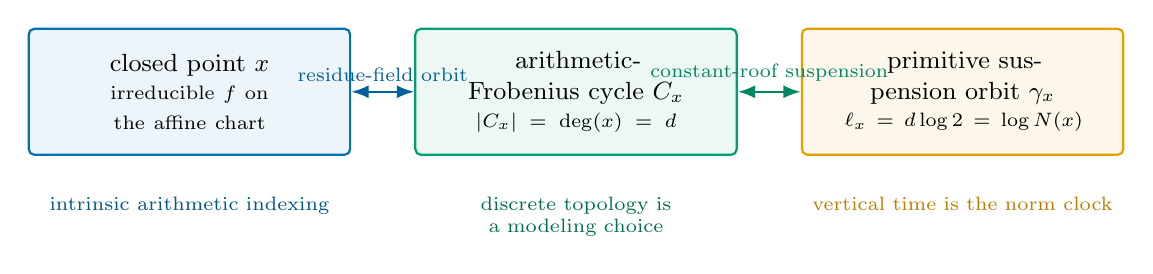
\begin{tikzpicture}[
  node distance=8mm and 8mm,
  every node/.style={font=\small,align=center},
  box/.style={draw,rounded corners=2pt,minimum height=16mm,text width=38mm,
              inner sep=4pt,line width=0.8pt},
  note/.style={font=\scriptsize,text width=38mm},
  link/.style={-{Latex[length=2.2mm]},line width=0.9pt},
  back/.style={{Latex[length=2.2mm]}-{Latex[length=2.2mm]},line width=0.9pt}
]
  \node[box,draw=FlowBlue,fill=FlowBlue!7] (closed)
    {closed point $x$\\[-1pt]
     \scriptsize irreducible $f$ on the affine chart};
  \node[box,draw=FlowTeal,fill=FlowTeal!7,right=of closed] (cycle)
    {arithmetic-Frobenius cycle $C_x$\\[-1pt]
     \scriptsize $|C_x|=\deg(x)=d$};
  \node[box,draw=FlowOrange,fill=FlowOrange!8,right=of cycle] (circle)
    {primitive suspension orbit $\gamma_x$\\[-1pt]
     \scriptsize $\ell_x=d\log 2=\log N(x)$};

  \draw[back,FlowBlue!85!black] (closed) -- node[above,font=\scriptsize]
    {residue-field orbit} (cycle);
  \draw[back,FlowTeal!85!black] (cycle) -- node[above,font=\scriptsize]
    {constant-roof suspension} (circle);

  \node[note,below=4mm of closed,text=FlowBlue!75!black]
    {intrinsic arithmetic indexing};
  \node[note,below=4mm of cycle,text=FlowTeal!70!black]
    {discrete topology is a modeling choice};
  \node[note,below=4mm of circle,text=FlowOrange!80!black]
    {vertical time is the norm clock};
\end{tikzpicture}

  \caption{The native three-way dictionary.  The closed point and its
  Frobenius cycle are arithmetic; the discrete topology used to form a
  locally compact suspension is disclosed separately.}
  \label{fig:dictionary}
\end{figure}

\section{Closed points become primitive flow circles}
\label{sec:orbits}

\subsection{The Frobenius ledger}

Closed points of the affine chart \(\mathbb A^1_{\F_2}\) correspond to monic
irreducible polynomials.  The point at infinity supplies one additional
rational closed point.  This concrete description agrees with the general
theorem that closed points over a finite field are Frobenius orbits on the
geometric points \citep[Sec.~1.4]{Deligne1974}.

\begin{lemma}[Exact cycle length]
\label{lem:cycle}
Let \(f\in\F_2[T]\) be monic and irreducible of degree \(d\), and let \(a\)
be one of its roots.  The points
\[
  a,a^2,a^{2^2},\ldots,a^{2^{d-1}}
\]
are distinct, form the full root set of \(f\), and constitute an
\(F\)-cycle of least length \(d\).
\end{lemma}

\begin{proof}
The residue field \(\F_2[T]/(f)\) is \(\F_{2^d}\), hence \(F^d(a)=a\).
If \(F^n(a)=a\), then \(a\in\F_{2^n}\).  The subfield
\(\F_2(a)=\F_{2^d}\) embeds in \(\F_{2^n}\), which forces \(d\mid n\).
Thus no smaller positive iterate fixes \(a\), and its \(d\) conjugates are
exactly the roots of \(f\).
\end{proof}

Let \(a_d\) denote the number of degree-\(d\) closed points of
\(\mathbb P^1_{\F_2}\).  Lemma~\ref{lem:cycle} gives
\begin{equation}
  a_1=3,
  \qquad
  a_d=\frac1d\sum_{e\mid d}\mu(e)2^{d/e}\qquad(d>1).
  \label{eq:closed-count}
\end{equation}
Every geometric point is defined over a finite extension, so every element of
\(S\) lies in one finite cycle.  If
\(N_n=\#\mathbb P^1(\F_{2^n})=2^n+1\), a cycle of exact size \(d\) contributes
all its \(d\) points to \(\Fix(F^n)\) precisely when \(d\mid n\).  Therefore
\begin{equation}
  N_n=2^n+1=\sum_{d\mid n}d\,a_d.
  \label{eq:fixed-ledger}
\end{equation}
This is the complete primitive-versus-repetition ledger on the discrete base.

\subsection{Circle decomposition and topology}

\begin{theorem}[Frobenius-suspension orbit dictionary]
\label{thm:dictionary}
For the frozen object there is a flow-preserving homeomorphism
\begin{equation}
  M_F\cong
  \coprod_{x\in|\mathbb P^1_{\F_2}|}
  \R/(\deg(x)\log2)\Z.
  \label{eq:circle-decomp}
\end{equation}
Consequently closed points, primitive Frobenius cycles, and primitive
suspension orbits are in bijection.  The orbit \(\gamma_x\) has least period
\begin{equation}
  \ell_x=\deg(x)\log2=\log(2^{\deg x})=\log N(x),
  \label{eq:period}
\end{equation}
and its \(r\)-fold traversal has period \(r\ell_x\).  Every flow point is
periodic, and the primitive ledger is locally finite by length.
\end{theorem}

\begin{proof}
Choose a root \(a\) in the cycle \(C_x\) and put \(d=\deg(x)\).  On the
suspension of that cycle define
\[
  \Psi_x([F^j a,u])=u+j\log2\pmod{d\log2}.
\]
Equation~\eqref{eq:action} replaces \((F^j a,u)\) by
\((F^{j+n}a,u-n\log2)\); both representatives have the same image.  Thus
\(\Psi_x\) is well defined.  It is a continuous bijection with the evident
continuous inverse and intertwines vertical translation.  Its coordinate
depends on the chosen root, but the component orbit and its period do not.
The least positive return requires exactly \(d\) base iterates, proving
\eqref{eq:period}.

Distinct Frobenius cycles are disjoint open-and-closed subsets because \(S\)
is discrete.  Below a length bound \(T\), only degrees
\(d\leq T/\log2\) occur, and there are finitely many closed points in each
such degree.  This proves completeness and local finiteness.
\end{proof}

The quotient also passes the elementary topological checks.  The \(\Z\)-action
is free because equality of real coordinates in
\eqref{eq:action} forces \(n\log2=0\).  It is properly discontinuous: the
real projection of a compact subset is bounded, and only finitely many
translates by \(n\log2\) can meet that bounded interval.  Hence the quotient
is locally compact and Hausdorff.  It is second countable because it is a
countable disjoint union of second-countable circles, and it is noncompact
because it has infinitely many open-and-closed components.

These positive properties should not be confused with chaotic dynamics.  The
flow has no nonzero transverse tangent direction, no stable or unstable
multiplier, no mixing, and no interaction between primitive components.  A
Poincar\'e section is zero-dimensional.  This degeneracy is central to the
later determinant distinction.

\section{Exact native zeta and endogenous weights}
\label{sec:zeta}

Artin and Mazur define the fixed-point zeta by
\begin{equation}
  \zeta_{AM}(z)
   =\exp\!\left(\sum_{n\geq1}\frac{N_n}{n}z^n\right)
  \label{eq:am}
\end{equation}
when the fixed-point counts are finite \citep[p.~84]{ArtinMazur1965}.
For a finite-field power map they identify this with the classical zeta.  The
following proof records exactly how the primitive cycle ledger enters.

\begin{theorem}[Orbit, Artin--Mazur, and Hasse--Weil identity]
\label{thm:zeta}
As formal power series in \(z\),
\begin{equation}
\begin{aligned}
  \zeta_{AM}(z)
   &=\prod_{d\geq1}(1-z^d)^{-a_d}\\
   &=\prod_{x\in|\mathbb P^1_{\F_2}|}
       (1-z^{\deg x})^{-1}\\
   &=Z(\mathbb P^1_{\F_2},z)
    =\frac1{(1-z)(1-2z)}.
\end{aligned}
\label{eq:three-zeta}
\end{equation}
After \(z=2^{-s}\), the identity becomes
\begin{equation}
  \boxed{
  \zeta_{\mathrm{orb}}(s)
  =Z(\mathbb P^1_{\F_2},2^{-s})
  =\frac1{(1-2^{-s})(1-2^{1-s})}.}
  \label{eq:boxed-zeta}
\end{equation}
It holds analytically by the Euler product on \(\Re s>1\), and the rational
expression supplies a meromorphic continuation beyond that domain.
\end{theorem}

\begin{proof}
Using \eqref{eq:fixed-ledger}, formal reindexing gives
\[
\begin{aligned}
 \sum_{n\geq1}\frac{N_n}{n}z^n
  &=\sum_{n\geq1}\frac{z^n}{n}\sum_{d\mid n}d a_d
    =\sum_{d\geq1}a_d\sum_{r\geq1}\frac{z^{rd}}r\\
  &=-\sum_{d\geq1}a_d\log(1-z^d).
\end{aligned}
\]
Each coefficient uses only finitely many divisors, so no analytic
rearrangement is hidden in this step.  Exponentiation gives the first two
equalities in \eqref{eq:three-zeta}.  The closed-point product is the
Hasse--Weil definition \citep[Sec.~1.1]{Deligne1974}.  Finally,
\[
  \exp\!\left(\sum_{n\geq1}\frac{(2^n+1)z^n}{n}\right)
  =\exp[-\log(1-2z)-\log(1-z)],
\]
which proves the rational expression.  Theorem~\ref{thm:dictionary} converts
\(z^{\deg x}\) into \(\e^{-s\ell_x}\).
\end{proof}

\begin{corollary}[Weight provenance]
\label{cor:weights}
On the absolute-convergence half-plane,
\begin{align}
  \log\zeta_{\mathrm{orb}}(s)
   &=\sum_x\sum_{r\geq1}\frac{N(x)^{-rs}}r,
  \label{eq:logzeta}\\
  -\frac{d}{ds}\log\zeta_{\mathrm{orb}}(s)
   &=\sum_x\sum_{r\geq1}\log N(x)\,N(x)^{-rs}.
  \label{eq:logderivative}
\end{align}
Thus \(1/r\) is forced by the logarithm of a primitive factor, while
\(\log N(x)=\ell_x\) is forced by differentiation with respect to suspension
time.
\end{corollary}

The result is positive but tightly scoped.  No sign, complex phase,
\(N(x)^{-r/2}\) amplitude, or stability denominator appears in
\eqref{eq:logderivative}.  Introducing a half-shift in \(s\) would change the
frozen normalization rather than reveal a latent term.  Replacing \(F\) with
\(F^{-1}\) leaves \eqref{eq:boxed-zeta} unchanged, so orientation reversal
cannot supply such a phase.

\begin{table}[t]
\centering
\caption{The first eight rows of the exact closed-point ledger.  The finite
table is a regression control; Equation~\eqref{eq:fixed-ledger} is the proof.}
\label{tab:ledger}
\small
\begin{tabular}{@{}rrrrr@{}}
\toprule
\(d\) & affine irreducibles & \(a_d\) on \(\mathbb P^1\) & \(2^d+1\) & \(\sum_{e\mid d}e a_e\)\\
\midrule
1 & 2 & 3 & 3 & 3\\
2 & 1 & 1 & 5 & 5\\
3 & 2 & 2 & 9 & 9\\
4 & 3 & 3 & 17 & 17\\
5 & 6 & 6 & 33 & 33\\
6 & 9 & 9 & 65 & 65\\
7 & 18 & 18 & 129 & 129\\
8 & 30 & 30 & 257 & 257\\
\bottomrule
\end{tabular}
\end{table}

\section{Convergence, continuation, and determinant types}
\label{sec:analytic}

\begin{theorem}[Exact absolute-convergence boundary]
\label{thm:convergence}
The logarithmic orbit expansion and primitive Euler product converge
absolutely exactly for \(\Re s>1\).
\end{theorem}

\begin{proof}
Put \(\sigma=\Re s\).  For \(\sigma>0\), positivity and
\eqref{eq:am} reduce absolute convergence to
\begin{equation}
  \sum_{n\geq1}\frac{(2^n+1)2^{-\sigma n}}n.
  \label{eq:convseries}
\end{equation}
The first part is \(\sum_n2^{(1-\sigma)n}/n\).  It converges for
\(\sigma>1\), becomes the harmonic series at \(\sigma=1\), and fails the
term test for \(0<\sigma<1\).  The second positive part cannot repair that
divergence.  For \(\sigma\leq0\), the primitive factors do not approach one
in the required manner (and may be singular), so absolute Euler-product
convergence also fails.
\end{proof}

The rational function in \eqref{eq:boxed-zeta} continues meromorphically to
all \(s\in\C\).  This does not mean that the defining Euler product converges
after continuation.  It also makes the single clock visible:
\begin{equation}
  \zeta_X\!\left(s+\frac{2\pi i k}{\log2}\right)=\zeta_X(s),
  \qquad k\in\Z.
  \label{eq:imag-period}
\end{equation}
The poles lie on the two lattices
\[
  s=\frac{2\pi i k}{\log2},
  \qquad
  s=1+\frac{2\pi i k}{\log2}.
\]
Writing \(Z(t)=((1-t)(1-2t))^{-1}\), direct algebra gives
\[
  Z\!\left(\frac1{2t}\right)=2t^2Z(t),
  \qquad
  \zeta_X(1-s)=2^{1-2s}\zeta_X(s).
\]
This is the native \(\mathbb P^1\) functional relation, not the completed
Riemann functional equation.

The scalar equality in Theorem~\ref{thm:zeta} passes through three logically
different constructions, summarized in Table~\ref{tab:determinants}.
Deligne's cohomological formula has the form
\begin{equation}
  Z(X,t)=\prod_i
  \det\!\left(I-t\Phi_{\mathrm{coh}}\mid
  H_c^i(X_{\overline{\F}_Q},\mathbb Q_\ell)\right)^{(-1)^{i+1}}.
  \label{eq:cohom-det}
\end{equation}
Here \(\Phi_{\mathrm{coh}}\) denotes the cohomological Frobenius in the
convention of the cited trace formula, commonly geometric Frobenius in Galois
notation.  It is deliberately not denoted by \(F\): the suspension return map
is the arithmetic point action \(a\mapsto a^Q\).  The two point permutations
are inverse and have the same finite cycles and fixed-point counts, but their
operator actions must not be conflated.  For \(\mathbb P^1/\F_2\), the
cohomological determinant factors are \(1-t\) and \(1-2t\).
It provides rational continuation, and Poincar\'e duality supplies the native
functional equation in the proper smooth setting
\citep[Secs.~1.5 and 2.6]{Deligne1974}; see also
\citep[Secs.~26--29]{Milne2013}.  Equation~\eqref{eq:cohom-det} acts on
\(\ell\)-adic cohomology.  It is not the determinant of a Poincar\'e return
derivative or a trace-class transfer operator of the circle flow.

\begin{table}[t]
\centering
\caption{Three native zeta constructions and the boundaries of their
identification.}
\label{tab:determinants}
\small
\begin{tabularx}{\textwidth}{@{}L{0.24\textwidth}Y L{0.25\textwidth}@{}}
\toprule
Construction & Defined from & What is proved\\
\midrule
Primitive-orbit Euler product & one factor per suspension circle & equals the native closed-point product\\
Artin--Mazur zeta & fixed-point counts \(N_n\) & equals the same formal series\\
Cohomological Frobenius determinant & \(\Phi_{\mathrm{coh}}\) on compactly supported \(\ell\)-adic cohomology & rationality and native analytic structure\\
Circle-flow transfer determinant & an operator and trace ideal not supplied here & \nottest\\
\bottomrule
\end{tabularx}
\end{table}

The equality of the first three scalar functions is explained by their common
arithmetic ledger.  An operator equivalence between the second or third and a
flow transfer operator would require a separately defined space, action,
domain, trace, and intertwining theorem.  None is implicit in the circle
decomposition.

\section{One clock cannot cross characteristics}
\label{sec:clock}

The fixed-field construction extends without parameter fitting to any fixed
variety over \(\F_Q\): arithmetic Frobenius cycles yield primitive periods
\(\deg(x)\log Q\).  Changing the variety alters multiplicities, but every
period remains in the lattice \((\log Q)\N\).  The following elementary
theorem locates the exact characteristic-zero obstruction.

\begin{theorem}[One-clock obstruction]
\label{thm:clock}
Let \(Q=\ell^f\), where \(\ell\) is a rational prime and \(f\geq1\).  If
positive integers \(n,r\) and a rational prime \(p\) satisfy
\begin{equation}
  n\log Q=r\log p,
  \label{eq:clock-equality}
\end{equation}
then \(p=\ell\) and \(fn=r\).  If
\(n\log Q=\log p\), then \(Q=p=\ell\) and \(f=n=1\).
\end{theorem}

\begin{proof}
Exponentiating \eqref{eq:clock-equality} gives
\(\ell^{fn}=p^r\).  Unique factorization in \(\Z\) forces \(p=\ell\),
after which equality of exponents yields \(fn=r\).  When \(r=1\), positivity
of \(f\) and \(n\) forces \(f=n=1\).
\end{proof}

\begin{figure}[t]
  \centering
  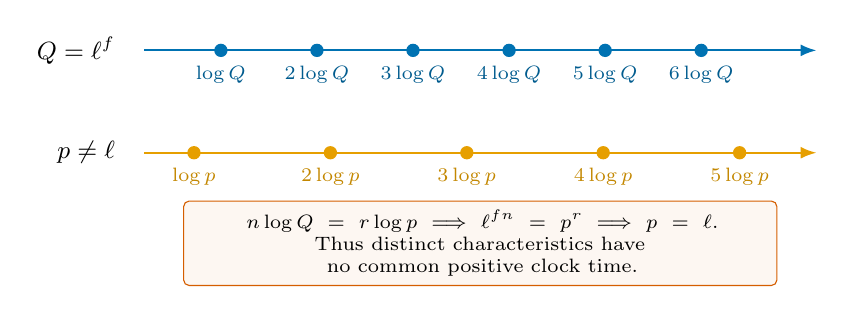
\begin{tikzpicture}[
  x=1.22cm,y=1cm,
  every node/.style={font=\scriptsize},
  tick/.style={circle,fill,inner sep=1.7pt},
  axis/.style={-{Latex[length=2mm]},line width=0.75pt},
  brace/.style={decorate,decoration={brace,amplitude=4pt}}
]
  \node[anchor=east,font=\small] at (0,2.2) {$Q=\ell^f$};
  \draw[axis,FlowBlue] (0.2,2.2) -- (7.2,2.2);
  \foreach \x/\lab in {1/$\log Q$,2/$2\log Q$,3/$3\log Q$,4/$4\log Q$,5/$5\log Q$,6/$6\log Q$}{
    \node[tick,FlowBlue] at (\x,2.2) {};
    \node[below=2pt,text=FlowBlue!80!black] at (\x,2.2) {\lab};
  }

  \node[anchor=east,font=\small] at (0,0.9) {$p\ne\ell$};
  \draw[axis,FlowOrange] (0.2,0.9) -- (7.2,0.9);
  \foreach \x/\lab in {0.72/$\log p$,2.14/$2\log p$,3.56/$3\log p$,4.98/$4\log p$,6.40/$5\log p$}{
    \node[tick,FlowOrange] at (\x,0.9) {};
    \node[below=2pt,text=FlowOrange!85!black] at (\x,0.9) {\lab};
  }
  \node[draw=FlowRed,rounded corners=2pt,fill=FlowRed!5,align=center,
        text width=73mm,font=\scriptsize] at (3.7,-0.25)
    {$n\log Q=r\log p\Longrightarrow \ell^{fn}=p^r
      \Longrightarrow p=\ell$.\\
     Thus distinct characteristics have no common positive clock time.};
\end{tikzpicture}

  \caption{Schematic clock lattices.  The placement is illustrative; the
  nonintersection statement follows from unique factorization, not from the
  drawing or a numerical spacing comparison.}
  \label{fig:clocks}
\end{figure}

The obstruction is an equality statement, not a rank or density comparison.
One may have accidental numerical proximity between unrelated logarithms, but
an exact period identity across distinct prime bases is impossible.  Passing
from one finite field to all rational primes therefore requires a new global
clock mechanism or an object that genuinely couples residue characteristics.
No larger variety over the same \(\F_Q\) can remove the lattice restriction.

There is also a purely analytic signature.  Every rational function of
\(Q^{-s}\) has the nonzero imaginary period \(2\pi i/\log Q\).  The rational
Euler product has no such fixed imaginary period on \(\Re s>1\).  Indeed, if
its absolutely convergent Dirichlet series were periodic by \(iT\), uniqueness
would force both \(2^{-iT}=1\) and \(3^{-iT}=1\).  Hence
\(T\log2,T\log3\in2\pi\Z\), which for nonzero \(T\) would imply an equality
\(2^a=3^b\) with positive integers \(a,b\), contradicting unique
factorization.  This distinguishes the analytic clocks without consulting
Riemann zeros.

\section{The exact repair that proves too much}
\label{sec:compiler}

The most tempting repair is to abandon one clock and give each rational prime
its own component.  It is better to state the universal theorem first.

\begin{theorem}[Universal Euler-product compiler]
\label{thm:compiler}
Let \(J\) be countable and let \(\{L_j:j\in J\}\subset(0,\infty)\) be locally
finite in length.  The translation flow on
\begin{equation}
  M_L=\coprod_{j\in J}\R/L_j\Z
  \label{eq:compiler-space}
\end{equation}
is locally compact, Hausdorff, and second countable, with exactly one
primitive orbit of length \(L_j\) on each component.  Wherever it converges,
\begin{equation}
  \zeta_{M_L}(s)=\prod_{j\in J}(1-\e^{-sL_j})^{-1}.
  \label{eq:compiler-product}
\end{equation}
\end{theorem}

\begin{proof}
The topological properties hold componentwise for the countable coproduct.
Local finiteness of \(\{L_j\}\) gives a finite primitive ledger below every
length cutoff.  Translation on one circle has the whole circle as one
primitive orbit, whose repetitions give the geometric factor in
\eqref{eq:compiler-product}.  Multiplication over components proves the
identity.
\end{proof}

Taking \(J\) to be the rational primes and \(L_p=\log p\) produces
\begin{equation}
  M_{\Z}^{\mathrm{taut}}
   =\coprod_p\R/(\log p)\Z,
  \qquad
  \zeta_{M_{\Z}^{\mathrm{taut}}}(s)=\zeta(s)
  \quad(\Re s>1).
  \label{eq:prime-compiler}
\end{equation}
The invariant-looking notation
\[
  \coprod_{x\in|\Spec\Z|}\R/(\log N(x))\Z
\]
does not alter the information flow.  Every target closed point and its norm
are queried before the corresponding component exists.  There is no coupled
return map whose periodic points generate the divisor.

Theorem~\ref{thm:compiler} works equally for composite-only lengths,
quadratic-irrational lengths, a randomized locally finite list, or a divisor
chosen from an unrelated function.  It therefore establishes an exact
proves-too-much control.  In Route-A language, the prime-circle flow has an
exact primitive ledger and an exact orbit product, but it fails A0 because
both the target labels and the \(\log p\) roofs are inputs.

The same-cycle-type control exposes a second limitation.  Let \(G\) be a
permutation of a countable discrete set for which every point is periodic and
whose number of cycles of each finite length equals that of \(F\).  Then \(G\)
is conjugate to \(F\) as a discrete dynamical system: match cycles one-by-one
and preserve cyclic order.  Its constant-roof suspension is therefore
flow-conjugate to \(M_F\) and has the same orbit zeta.  The periodicity
hypothesis is essential: additional infinite orbits would be additional
components not present in the frozen Frobenius system.  The bare flow topology
remembers the sequence \((a_d)\), but it does not recover the algebraic
geometry or \(\ell\)-adic cohomology that generated those counts.

\begin{figure}[t]
  \centering
  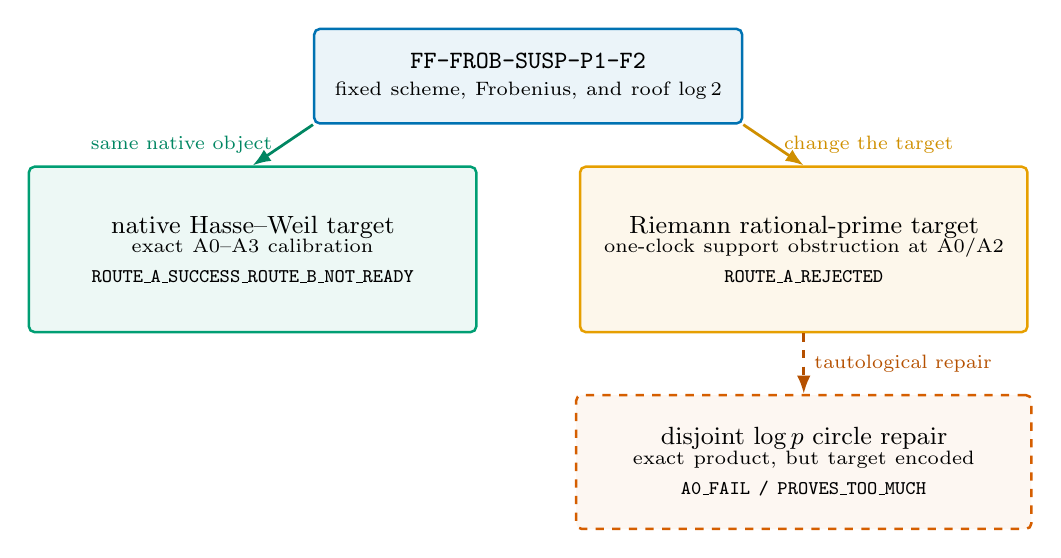
\begin{tikzpicture}[
  every node/.style={font=\small,align=center},
  source/.style={draw,rounded corners=2pt,minimum height=12mm,text width=52mm,
                 fill=FlowBlue!8,draw=FlowBlue,line width=0.9pt},
  outcome/.style={draw,rounded corners=2pt,minimum height=21mm,text width=54mm,
                  inner sep=4pt,line width=0.9pt},
  control/.style={draw,dashed,rounded corners=2pt,minimum height=17mm,text width=55mm,
                  inner sep=4pt,line width=0.9pt},
  arr/.style={-{Latex[length=2.3mm]},line width=1pt}
]
  \node[source] (src) at (0,0)
    {\texttt{FF-FROB-SUSP-P1-F2}\\[-1pt]
     \scriptsize fixed scheme, Frobenius, and roof $\log 2$};
  \node[outcome,draw=FlowTeal,fill=FlowTeal!7] (native) at (-3.5,-2.2)
    {native Hasse--Weil target\\[-1pt]
     \scriptsize exact A0--A3 calibration\\
     \scriptsize \texttt{ROUTE\_A\_SUCCESS\_ROUTE\_B\_NOT\_READY}};
  \node[outcome,draw=FlowOrange,fill=FlowOrange!8] (riemann) at (3.5,-2.2)
    {Riemann rational-prime target\\[-1pt]
     \scriptsize one-clock support obstruction at A0/A2\\
     \scriptsize \texttt{ROUTE\_A\_REJECTED}};
  \node[control,draw=FlowRed,fill=FlowRed!5] (compiler) at (3.5,-4.9)
    {disjoint $\log p$ circle repair\\[-1pt]
     \scriptsize exact product, but target encoded\\
     \scriptsize \texttt{A0\_FAIL / PROVES\_TOO\_MUCH}};

  \draw[arr,FlowTeal!85!black] (src.south west) -- node[left,font=\scriptsize]
    {same native object} (native.north);
  \draw[arr,FlowOrange!90!black] (src.south east) -- node[right,font=\scriptsize]
    {change the target} (riemann.north);
  \draw[arr,dashed,FlowRed!85!black] (riemann.south) -- node[right,font=\scriptsize]
    {tautological repair} (compiler.north);
\end{tikzpicture}

  \caption{Target-specific Route-A fork.  Exact native success does not
  transfer to the Riemann target, and the disjoint repair is rejected at the
  arithmetic-origin gate despite exact scalar matching.}
  \label{fig:fork}
\end{figure}

\section{Target-specific Route-A assessment}
\label{sec:route}

A verdict without a named target would merge two incompatible claims.  The
native finite-field zeta and the Riemann zeta are therefore evaluated in
separate columns, with the compiler retained as an adversarial control.

\begin{table}[t]
\centering
\caption{Route-A assessment.  Later-layer exactness cannot repair a failed
arithmetic-origin gate.}
\label{tab:route}
\small
\begin{tabularx}{\textwidth}{@{}L{0.075\textwidth}YYY@{}}
\toprule
Layer & Native \(Z(\mathbb P^1/\F_2)\) & Same flow, Riemann target & Disjoint-prime compiler\\
\midrule
A0 & \texttt{ANALYTIC\_\allowbreak ARITHMETIC\_\allowbreak ORIGIN} & \texttt{FAIL}: one characteristic & \texttt{FAIL}: target encoded\\
A1 & \texttt{PASS\_ANALYTIC} & exact flow ledger, wrong support & \texttt{PASS\_ANALYTIC}\\
A2 & \texttt{ANALYTIC\_DETERMINANT} & \texttt{FAIL}: wrong product and clock & exact only tautologically\\
A3 & \texttt{CONTROLLED\_CONTINUATION} & \texttt{FAIL}: incompatible global structure & \texttt{FAIL}: no dynamical provenance\\
A4 & \texttt{FAIL / NOT\_TESTABLE} & \texttt{FAIL / NOT\_TESTABLE} & \texttt{FAIL / NOT\_TESTABLE}\\
Overall & \texttt{SUCCESS\_\allowbreak ROUTE\_B\_\allowbreak NOT\_READY}, native calibration only & \texttt{ROUTE\_A\_\allowbreak REJECTED} & \texttt{REJECTED / \allowbreak PROVES\_TOO\_MUCH}\\
\bottomrule
\end{tabularx}
\end{table}

For the native target, A0 is analytic because the scheme and its Frobenius
generate the closed-point ledger before the zeta is evaluated.  A1 is analytic
because primitive cycles, repetitions, orientation, multiplicity,
completeness, and local finiteness are exact.  A2 records an exact
orbit-zeta identity, not a trace-class operator theorem.  A3 records native
rational continuation and the functional relation with their cohomological
source named.  A4 fails because no natural quantization, unitary completion,
or scattering lift has been defined.

For the Riemann target, A0 fails by Theorem~\ref{thm:clock}.  The orbit ledger
still exists, but it carries the wrong primitive support.  A2 fails because
the determinant is the wrong Euler product and has the wrong single-clock
periodicity.  A3 lacks the Riemann gamma factor, pole removal, counting law,
and an intrinsic Weil-form compression.  A4 again has no candidate lift.
The overall status is \texttt{ROUTE\_A\_REJECTED}.

For the compiler, A1 and the formal orbit product are exact only because the
desired index set and lengths were supplied as input.  The construction
receives \texttt{A0\_FAIL} and
\texttt{STOP\_SCOPED / PROVES\_TOO\_MUCH}.  This is precisely why scalar zeta
matching is subordinate to arithmetic provenance.

No object in this paper has \texttt{route\_b\_invocation\_allowed: true}.
No B1--B5 evaluation is performed, and no self-adjoint or Hilbert--P\'olya
claim is inferred from the finite-field calibration.

\section{Deterministic controls}
\label{sec:controls}

The companion Python program checks the proof ledger with exact integer and
finite-polynomial arithmetic.  A polynomial over \(\F_2\) is encoded by its
coefficient bits.  Monic polynomials through degree 12 are enumerated, and
irreducibility is certified by the Frobenius--Rabin criterion: for a monic
degree-\(d\) polynomial \(f\), the program checks
\(T^{2^d}\equiv T\pmod f\) and the required gcd conditions for prime divisors
of \(d\).  It then adds the point at infinity in degree one.

The run examined 8190 monic polynomials, found 747 affine irreducibles, and
therefore recorded 748 projective closed points through degree 12.  Every
enumerated count equals the M\"obius formula, and every fixed-point count
\(2^n+1\) is recovered from primitive cycles.  The formal orbit product and
\(1/((1-z)(1-2z))\) have identical coefficients through the frozen order;
the coefficient at \(z^n\) is \(2^{n+1}-1\).  A separate ledger records each
pair \((d,r)\), retaining \(1/r\) and \(d\log2\) as distinct sources.

Further controls evaluate finite partial Euler logs on both sides of
\(\Re s=1\), verify \eqref{eq:imag-period} to floating-point tolerance, and
exhaust a finite grid of clock equalities generated at runtime.  All 90 grid
solutions use the same characteristic and satisfy the exponent identity
\(fn=r\).  Finally, composite-only, integer-log, and
quadratic-irrational circle profiles reproduce their encoded products just as
the prime-circle construction does.

\begin{table}[t]
\centering
\caption{Deterministic control suite and evidentiary boundary.}
\label{tab:controls}
\small
\begin{tabularx}{\textwidth}{@{}L{0.29\textwidth}L{0.20\textwidth}Y@{}}
\toprule
Control & Result & Interpretation\\
\midrule
Unit tests & 13/13 pass & implementation integrity\\
M\"obius versus enumeration & all degrees 1--12 match & finite exact regression\\
Fixed points from cycles & all degrees 1--12 match & primitive/repetition separation\\
Formal zeta coefficients & orders 0--12 match & finite check of an independently proved identity\\
Clock grid & 90/90 solutions same-characteristic & finite check of Theorem~\ref{thm:clock}\\
Imaginary periodicity & maximum displayed error below \(3.0\times10^{-14}\) & floating-point software check\\
Unrelated circle profiles & encoded and orbit products agree & proves-too-much control\\
\bottomrule
\end{tabularx}
\end{table}

These computations do not upgrade a theorem's evidence status.  They use no
Riemann-zero locations, fitted scale or shift, random seed, network data, or
hard-coded rational-prime table.  Primes needed for the finite
same-characteristic grid are generated by trial division at runtime.  From
the paper directory, the full suite is reproduced with
\begin{verbatim}
bash experiments/reproduce.sh
\end{verbatim}

\section{Discussion}
\label{sec:discussion}

The Frobenius suspension succeeds at the interface that failed for less
structured orbit proposals: it has one primitive arithmetic object per
primitive flow orbit, an exact return clock, endogenous repetitions, and a
closed-form zeta.  Nothing is inferred from a fitted spectral statistic.
This makes it a clean finite-field calibration for evaluating more ambitious
arithmetic flows.

The calibration also exposes a boundary.  The statement that closed points
resemble periodic orbits is not yet a characteristic-zero construction.  Over one finite field, every
norm is a power of one base \(Q\).  A constant roof converts degree into
\(\log N(x)\) because \(N(x)=Q^{\deg x}\).  Over \(\Spec\Z\), closed-point
norms have different prime bases.  Theorem~\ref{thm:clock} says that the
difference is not repaired by increasing degree, changing multiplicities, or
choosing a larger variety over the same field.

The hostile objection to the positive control is valid: after imposing the
discrete topology, the suspension is an orbit ledger in geometric dress.  An
arbitrary permutation with the same cycle counts produces the same bare flow.
The construction does not retain Zariski incidence, a transverse derivative,
or cohomology as intrinsic topology of the circle union.  Its value lies in
making every normalization decision visible and exact, not in supplying
dynamical complexity.

The determinant taxonomy sharpens the next problem.  The orbit product and
the cohomological determinant agree as functions because both read the same
closed-point counts.  A same-object operator bridge would have to explain how
the circle dynamics acts on a trace domain whose fixed-point coefficients
recover the cohomological expression.  Equality of scalar outputs alone does
not construct that bridge.  In particular, no stability factor or signed
phase can be borrowed from \(\ell\)-adic cohomology and then described as a
return derivative of a zero-dimensional transverse section.

The universal compiler gives a practical falsification rule for future
proposals.  If replacing the purported arithmetic objects by any locally
finite length list leaves the proof unchanged, the proof establishes
realizability, not arithmetic emergence.  The next construction must therefore
couple residue characteristics before its primitive ledger is known.  It must
derive \(\log N(x)\) as a return time from one global mechanism, and it must
possess a topology or trace framework that does more than take a coproduct of
already labeled circles.

One precise next theorem obligation is consequently available:
construct a single non-disjoint arithmetic phase space across residue
characteristics with (i) an intrinsic return map generating its primitive
closed objects, (ii) an emergent norm clock, (iii) a locally compact or
otherwise trace-controlled global structure, and (iv) an exact test that
distinguishes it from Theorem~\ref{thm:compiler}.  Determinant or quantum
analysis should wait until those four clauses are satisfied.

\section{Limitations}
\label{sec:limitations}

The discrete topology on \(X(\overline{\F}_2)\) is imposed.  It is useful
because it makes the suspension locally compact and completely explicit, but
it suppresses algebraic adjacency and does not arise as the usual topology of
the scheme.  The resulting flow is disconnected and neutral: every component
is one periodic circle, all points are periodic, and there is no transverse
hyperbolicity or mixing.

Equation~\eqref{eq:orbit-zeta} defines an orbit Euler product, not a
trace-class flow operator.  This paper constructs no transfer space, nuclear
operator, wave trace, or Lefschetz complex for the suspension.  The
cohomological determinant in \eqref{eq:cohom-det} belongs to the algebraic
variety and Frobenius action.  An operator-level identification with the flow
remains \nottest.

The native finite-field continuation and functional relation do not provide a
Riemann gamma factor, Riemann--von Mangoldt counting law, Weil compression,
unitary lift, self-adjoint generator, or spectral determinant.  The
one-clock theorem rejects this frozen candidate for rational-prime support,
but it is not a no-go theorem for every possible arithmetic dynamics across
characteristics.  The computation cutoff at degree 12 is only a software
regression bound; none of the exact conclusions depends on it.

\section{Conclusion}

Arithmetic Frobenius on \(\mathbb P^1/\F_2\), after a disclosed
discrete-topology choice and constant-roof suspension, gives an exact native
finite-field positive control.  Closed points are primitive flow orbits,
their periods are \(\log N(x)\), and the orbit, Artin--Mazur, and Hasse--Weil
zetas agree with internally derived repetition and logarithmic weights.

The same proof determines the boundary.  A single \(Q\)-clock sees only its
own characteristic, while disjoint \(\log p\) circles merely compile the
target Euler product.  The native control therefore passes Route A only in
its stated finite-field scope; the Riemann target is rejected, and no Route-B
or Hilbert--P\'olya conclusion follows.

\section*{Reproducibility and declarations}

\paragraph{Data and code availability.}
All source-audit notes, proof records, deterministic Python code, tests,
generated tables, checksums, TikZ figure sources, bibliography, and manuscript
source are included in the \path{papers/4-arith-flow/} directory.  No external
dataset or Riemann-zero dataset was created or analyzed.

\paragraph{Ethics statement.}
This theoretical and computational study involves no human participants,
animals, intervention, personal data, or identifiable information.  No
institutional ethics review was required.

\paragraph{CRediT authorship contribution statement.}
Liang Wang: Conceptualization, Methodology, Formal analysis, Investigation,
Software, Validation, Data curation, Visualization, Writing---original draft,
and Writing---review and editing.

\paragraph{Funding.}
No project-specific external funding source was declared for this work.

\paragraph{Conflict of interest.}
The author declares no financial or non-financial conflict of interest
relevant to this study.

\paragraph{AI-assistance disclosure.}
OpenAI Codex assisted with source triage, deterministic implementation,
source-to-claim auditing, adversarial proof checking, figure preparation, and
manuscript drafting.  No generative system is credited as an author.  The
named author is responsible for source verification, mathematical claims,
artifact release, and the final text.

\appendix

\section{Finite-polynomial control}

The implementation represents
\(f(T)=\sum_jc_jT^j\in\F_2[T]\) by the integer whose \(j\)-th bit is \(c_j\).
Addition and subtraction are bitwise exclusive-or.  Multiplication is the
shift-and-exclusive-or algorithm, followed by polynomial long division when a
modulus is present.  For a monic polynomial of degree \(d\), the
Frobenius--Rabin criterion used in the control suite is
\[
  T^{2^d}\equiv T\pmod f,
  \qquad
  \gcd\!\left(f,T^{2^{d/q}}-T\right)=1
  \quad\text{for every prime }q\mid d.
\]
This supplies an independent constructive enumeration of the primitive
affine closed points.  The code also compares the count against
Equation~\eqref{eq:closed-count}; agreement is required at every degree, so a
bug in either enumeration or number-theoretic counting is exposed rather than
averaged away.

The formal product is multiplied coefficientwise through order 12.  For
\((1-z^d)^{-a_d}\), the coefficient of \(z^{rd}\) is
\(\binom{a_d+r-1}{r}\).  Truncated polynomial multiplication then gives the
orbit-product series.  The independent rational-function coefficient is
\(2^{n+1}-1\) at order \(n\).  The proof in
Theorem~\ref{thm:zeta} remains logically prior to this finite comparison.

\section{Claim-to-evidence ledger}

\begin{longtable}{@{}L{0.38\textwidth}L{0.18\textwidth}L{0.36\textwidth}@{}}
\caption{Status of the central manuscript claims.}\label{tab:claims}\\
\toprule
Claim & Evidence & Basis\\
\midrule
\endfirsthead
\toprule
Claim & Evidence & Basis\\
\midrule
\endhead
closed points are Frobenius cycles & \proved & primary source plus Lemma~\ref{lem:cycle}\\
cycle size equals residue degree & \proved & Lemma~\ref{lem:cycle}\\
suspension component is a circle of length \(d\log2\) & \proved & Theorem~\ref{thm:dictionary}\\
quotient is LCH, Hausdorff, and second countable & \proved{} after \modelchoice & direct topology proof\\
orbit, Artin--Mazur, and Hasse--Weil zetas agree & \proved & Theorem~\ref{thm:zeta}\\
\(1/r\) and \(\log N(x)\) are endogenous & \proved & Corollary~\ref{cor:weights}\\
absolute convergence is exactly \(\Re s>1\) & \proved & Theorem~\ref{thm:convergence}\\
one fixed finite-field clock covers all rational primes & \refuted & Theorem~\ref{thm:clock}\\
disjoint circles compile any locally finite length product & \proved & Theorem~\ref{thm:compiler}\\
circle flow is operator-equivalent to \(\ell\)-adic cohomology & \nottest & no operator map or trace theorem\\
construction supplies a Riemann gamma factor or half-weight & \refuted{} for frozen object & absent from source lock\\
natural quantum lift exists & \nottest & no Hilbert space, operator, or domain defined\\
\bottomrule
\end{longtable}

\section{Artifact map}

\begin{longtable}{@{}L{0.39\textwidth}L{0.53\textwidth}@{}}
\toprule
Relative path & Purpose\\
\midrule
\endfirsthead
\toprule
Relative path & Purpose\\
\midrule
\endhead
\path{notes/research_protocol.md} & frozen question, obligations, evidence vocabulary, and controls\\
\path{notes/source_audit.md} & verified primary-source corpus and claim boundaries\\
\path{notes/candidate_lock.md} & immutable object, clock, topology, zeta convention, and target split\\
\path{notes/proof_audit.md} & theorem proofs, adversarial controls, and dual Route-A verdict\\
\path{notes/composition_blueprint.md} & source-to-claim map and manuscript architecture\\
\path{code/frobenius_suspension_controls.py} & deterministic polynomial, zeta, clock, and compiler controls\\
\path{code/test_frobenius_suspension_controls.py} & 13 regression tests\\
\path{experiments/reproduce.sh} & one-command reproduction entry point\\
\path{results/closed_point_ledger.csv} & degree counts, fixed-point reconstruction, and periods\\
\path{results/zeta_formal_series_identity.csv} & finite formal-series identity\\
\path{results/repetition_weight_ledger.csv} & primitive-versus-repeated contribution ledger\\
\path{results/euler_product_convergence_controls.csv} & finite convergence regressions\\
\path{results/imaginary_periodicity_controls.csv} & software check of the single imaginary clock\\
\path{results/clock_intersection_controls.csv} & generated finite instances of the one-clock theorem\\
\path{results/universal_circle_compiler_controls.csv} & unrelated target-encoding controls\\
\path{results/frobenius_suspension_manifest.json} & parameters, interpretation boundary, verdicts, and SHA-256 hashes\\
\path{paper/figures/} & source-native TikZ diagrams\\
\bottomrule
\end{longtable}

\begingroup
\small
\bibliographystyle{plainnat}
\bibliography{references}
\endgroup

\end{document}
